A different way of encoding spikes is using a \emph{rank-order}; this means
keep just the order in which those spikes were fired and disregard the exact timing. Rank-ordered spike trains have been used in vision tasks under a biological plausibility constraint, making them a viable way of image encoding for neural applications~[\cite{van-rullen-rate-coding,basab-model,Masmoudi2010}].

Rank-ordered encoding is performed using an algorithm known as 
\emph{Filter overlap Correction algorithm} or \textbf{FoCal}~[\cite{basab-model}]. It models the \emph{foveal pit} region, the highest resolution area of the retina, with four ganglion cell layers that show a \emph{centre-surround} behaviour~[\cite{Kolb2003}]. In order to simulate these layers, four discrete 2D convolutions are performed. The centre-surround behaviour of the ganglion cells is modelled using Differences of Gaussians (DoG, Eq.~\ref{eq-dog}). 
\begin{equation}
\label{eq-dog}
DoG_w(x,y) = \pm\frac{1}{2\pi\sigma_{w,c}^2}e^{\frac{-(x^2 + y^2)}{2\sigma_{w,c}^2}}
\mp\frac{1}{2\pi\sigma_{w,s}^2}e^{\frac{-(x^2 + y^2)}{2\sigma_{w,s}^2}}
\end{equation}
where $\sigma_{w,c}$ and $\sigma_{w,s}$ are the standard deviation for the 
centre and surround components of the DoG at layer $w$. The signs 
will be ($-$,$+$) if the ganglion cell has an \textsc{off}-centre behaviour and 
($+$,$-$) if it has an \textsc{on}-centre one. Table~\ref{tab-kernel-specs} 
describes the parameters used to compute the convolution \emph{kernels} at each 
scale $w$.

\begin{table}[htb]
 \caption{Simulation parameters for ganglion cells}
  \begin{center}


  \bgroup
  \def\arraystretch{1.4}
      
  \begin{tabular}{c c c c c c}
    \begin{minipage}{0.7cm}\centering Layer \end{minipage}& 
    \begin{minipage}{0.8cm}\centering Centre \\type \end{minipage}& 
    \begin{minipage}{0.7cm} \centering Matrix width \end{minipage}&  
    \begin{minipage}{1.3cm}\centering Centre std. dev. ($\sigma_c$)\vspace*{0.1cm}\end{minipage} & 
    \begin{minipage}{1.3cm}\centering Surround std. dev. ($\sigma_s$)\vspace*{0.1cm}\end{minipage} & 
    \begin{minipage}{1.3cm}\centering Sampling resolution (cols,rows)\vspace*{0.1cm}\end{minipage} \\
    \hline
    \begin{minipage}{0.7cm}\centering 1  \end{minipage} &
    \begin{minipage}{0.8cm}\centering off \vspace*{0.005cm} \end{minipage}& 
    \begin{minipage}{0.7cm}\centering$3$ \end{minipage}& 
    $0.8$ & $6.7 \times \sigma_c$ &  1, 1 \\
    \begin{minipage}{0.7cm}\centering 2 \end{minipage} & 
    \begin{minipage}{0.8cm}\centering on \vspace*{0.005cm}\end{minipage} & 
    \begin{minipage}{0.7cm}\centering $11$ \end{minipage}& 
    $1.04$ & $6.7 \times \sigma_c$ & 1, 1 \\
    \begin{minipage}{0.7cm}\centering3 \end{minipage} &
    \begin{minipage}{0.8cm}\centering off \vspace*{0.005cm}\end{minipage} & 
    \begin{minipage}{0.7cm}\centering $61$ \end{minipage}& 
    $8$ & $4.8 \times \sigma_c$ & 5, 3 \\
    \begin{minipage}{0.7cm}\centering 4  \end{minipage} & 
    \begin{minipage}{0.8cm}\centering on \vspace*{0.005cm}\end{minipage} & 
    \begin{minipage}{0.7cm}\centering $243$\end{minipage} &
    $10.4$ & $4.8 \times \sigma_c$ & 5, 3 
  \end{tabular}
  \egroup
 \end{center}
  \label{tab-kernel-specs}
\end{table}

Every pixel value in the convolved images (Fig. \ref{fig-convolution-results}) 
is inversely proportional to a spike emission time (i.e. the higher the pixel value, the sooner the spike will be sent out.)

\begin{figure}[hbt]
  \centering
  \subfloat[Original image]{
    \label{sfig-rank-ordered-original}
    
\includegraphics[width=0.15\textwidth]{original_21-0}
  }
  \subfloat[Layer 1 (\textsc{off}-centre)]{
    \label{sfig-rank-ordered-midget-off}
    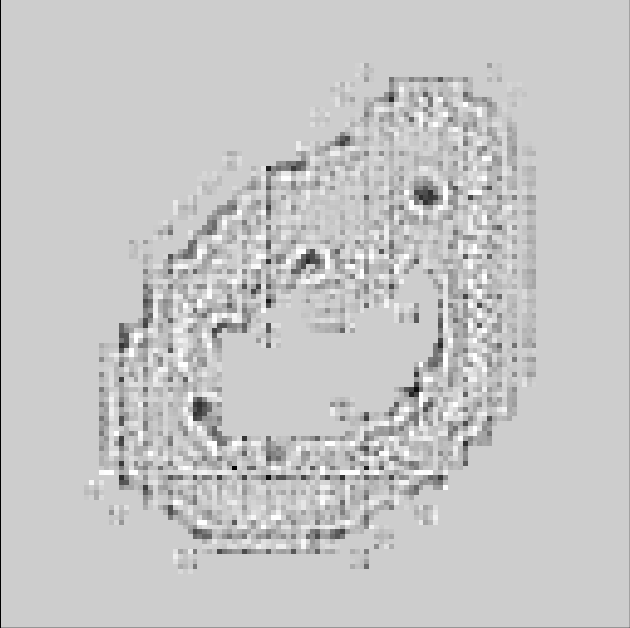
\includegraphics[width=0.15\textwidth]{filtered-21-0-layer-0}
  }
  \subfloat[Layer 2 (\textsc{on}-centre)]{
    \label{sfig-rank-ordered-midget-on}
    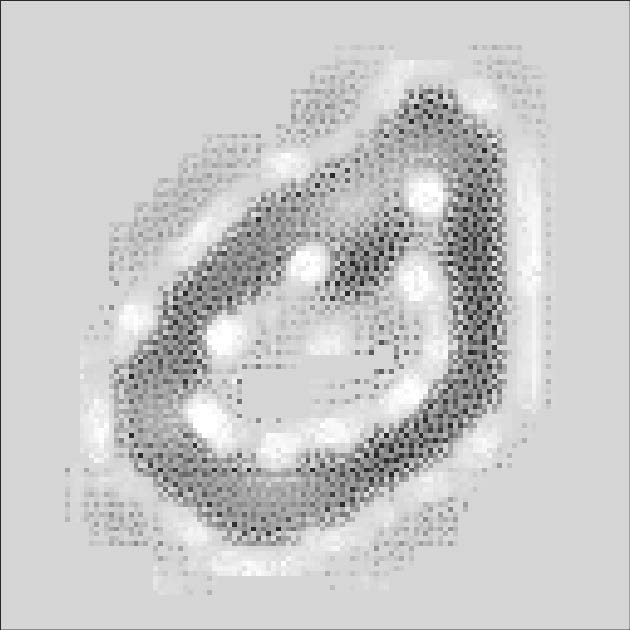
\includegraphics[width=0.15\textwidth]{filtered-21-0-layer-1}
  }\\
  \subfloat[Layer 3 (\textsc{off}-centre)]{
    \label{pic-lena-P-OFF}
    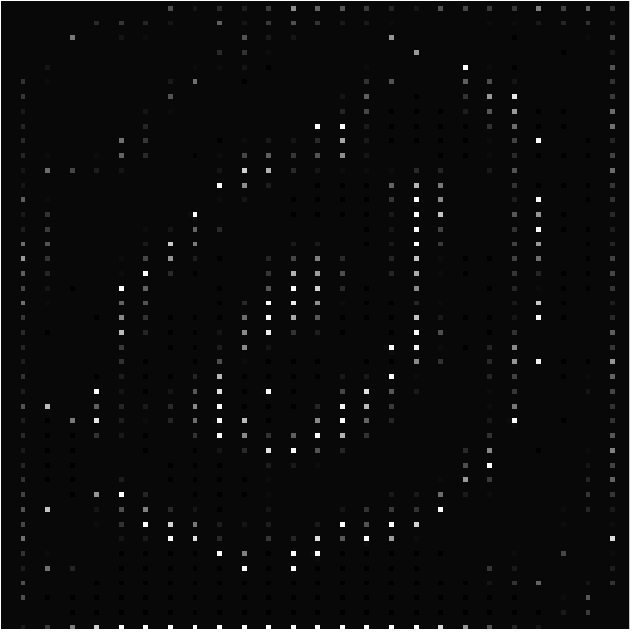
\includegraphics[width=0.15\textwidth]{filtered-21-0-layer-2}
  }
  \subfloat[Layer 4 (\textsc{on}-centre)]{
    \label{pic-lena-P-ON}
    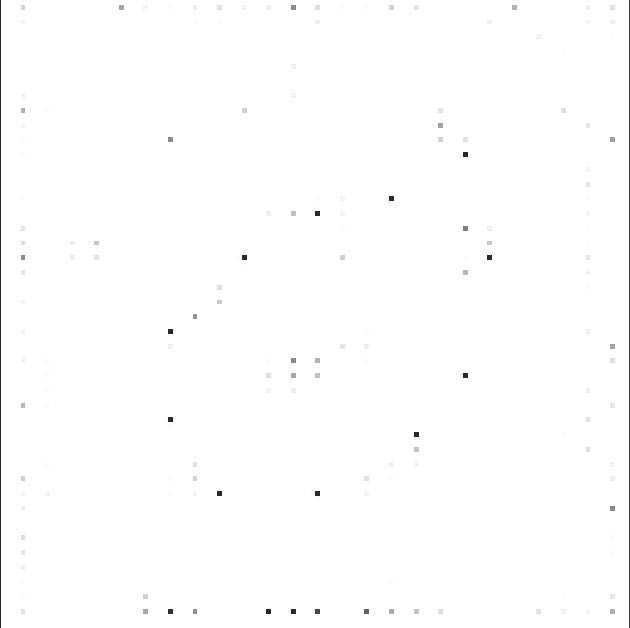
\includegraphics[width=0.15\textwidth]{filtered-21-0-layer-3}
  }
  \caption{Results of simulating ganglion cell layers and correcting for redundancy (convolved images are enhanced for better contrast).}
  \label{fig-convolution-results}
\end{figure}
The algorithm also performs a redundancy correction step; it does so by 
adjusting the convolved image's pixel value according to the correlation 
between convolution kernels (Alg.~\ref{code-focal-corr}).
\begin{algorithm}[h]
  \caption{FoCal, Part 2}
  \label{code-focal-corr}
  \begin{algorithmic}
    \Procedure{Correction}{coeffs $C$, correlations $Q$}
    \State $N \leftarrow \emptyset$ \Comment{Corrected coefficients}
    \Repeat
    \State $m \leftarrow max(C)$\Comment{Obtain maximum from $C$}
    \State $M \leftarrow M \cup m$\Comment{Add maximum to $M$}
    \State $C \leftarrow C \setminus m$\Comment{Remove maximum from $C$}
    \ForAll{$ c \in C$} \Comment{Adjust all remaining $c$}
    \If{$Q(m, c) \neq 0$} \Comment{Adjust only near}
    \State $c \leftarrow c - m \times Q(m, c)$
    \EndIf
    \EndFor
    \Until{$C = \emptyset$}
    \State \textbf{return} $M$
    \EndProcedure
  \end{algorithmic}
\end{algorithm}

After the correction step, the most important information can be recovered using only the first 30\% of the spikes. These significant spikes are shown in Figure~\ref{fig-raster-plot-30pc}, assuming that each spike will be generated 1~ms apart. One of the main advantages of ROC is that neurons will only spike once. Figure~\ref{fig-sorted-raster-plot-30pc} illustrates this fact and it also shows that not all simulated neurons fire, just the ones that encode useful information.
\begin{figure}[hbt]
  \centering
  \subfloat[First 30\% of generated spikes.]{
    \label{fig-raster-plot-30pc}
    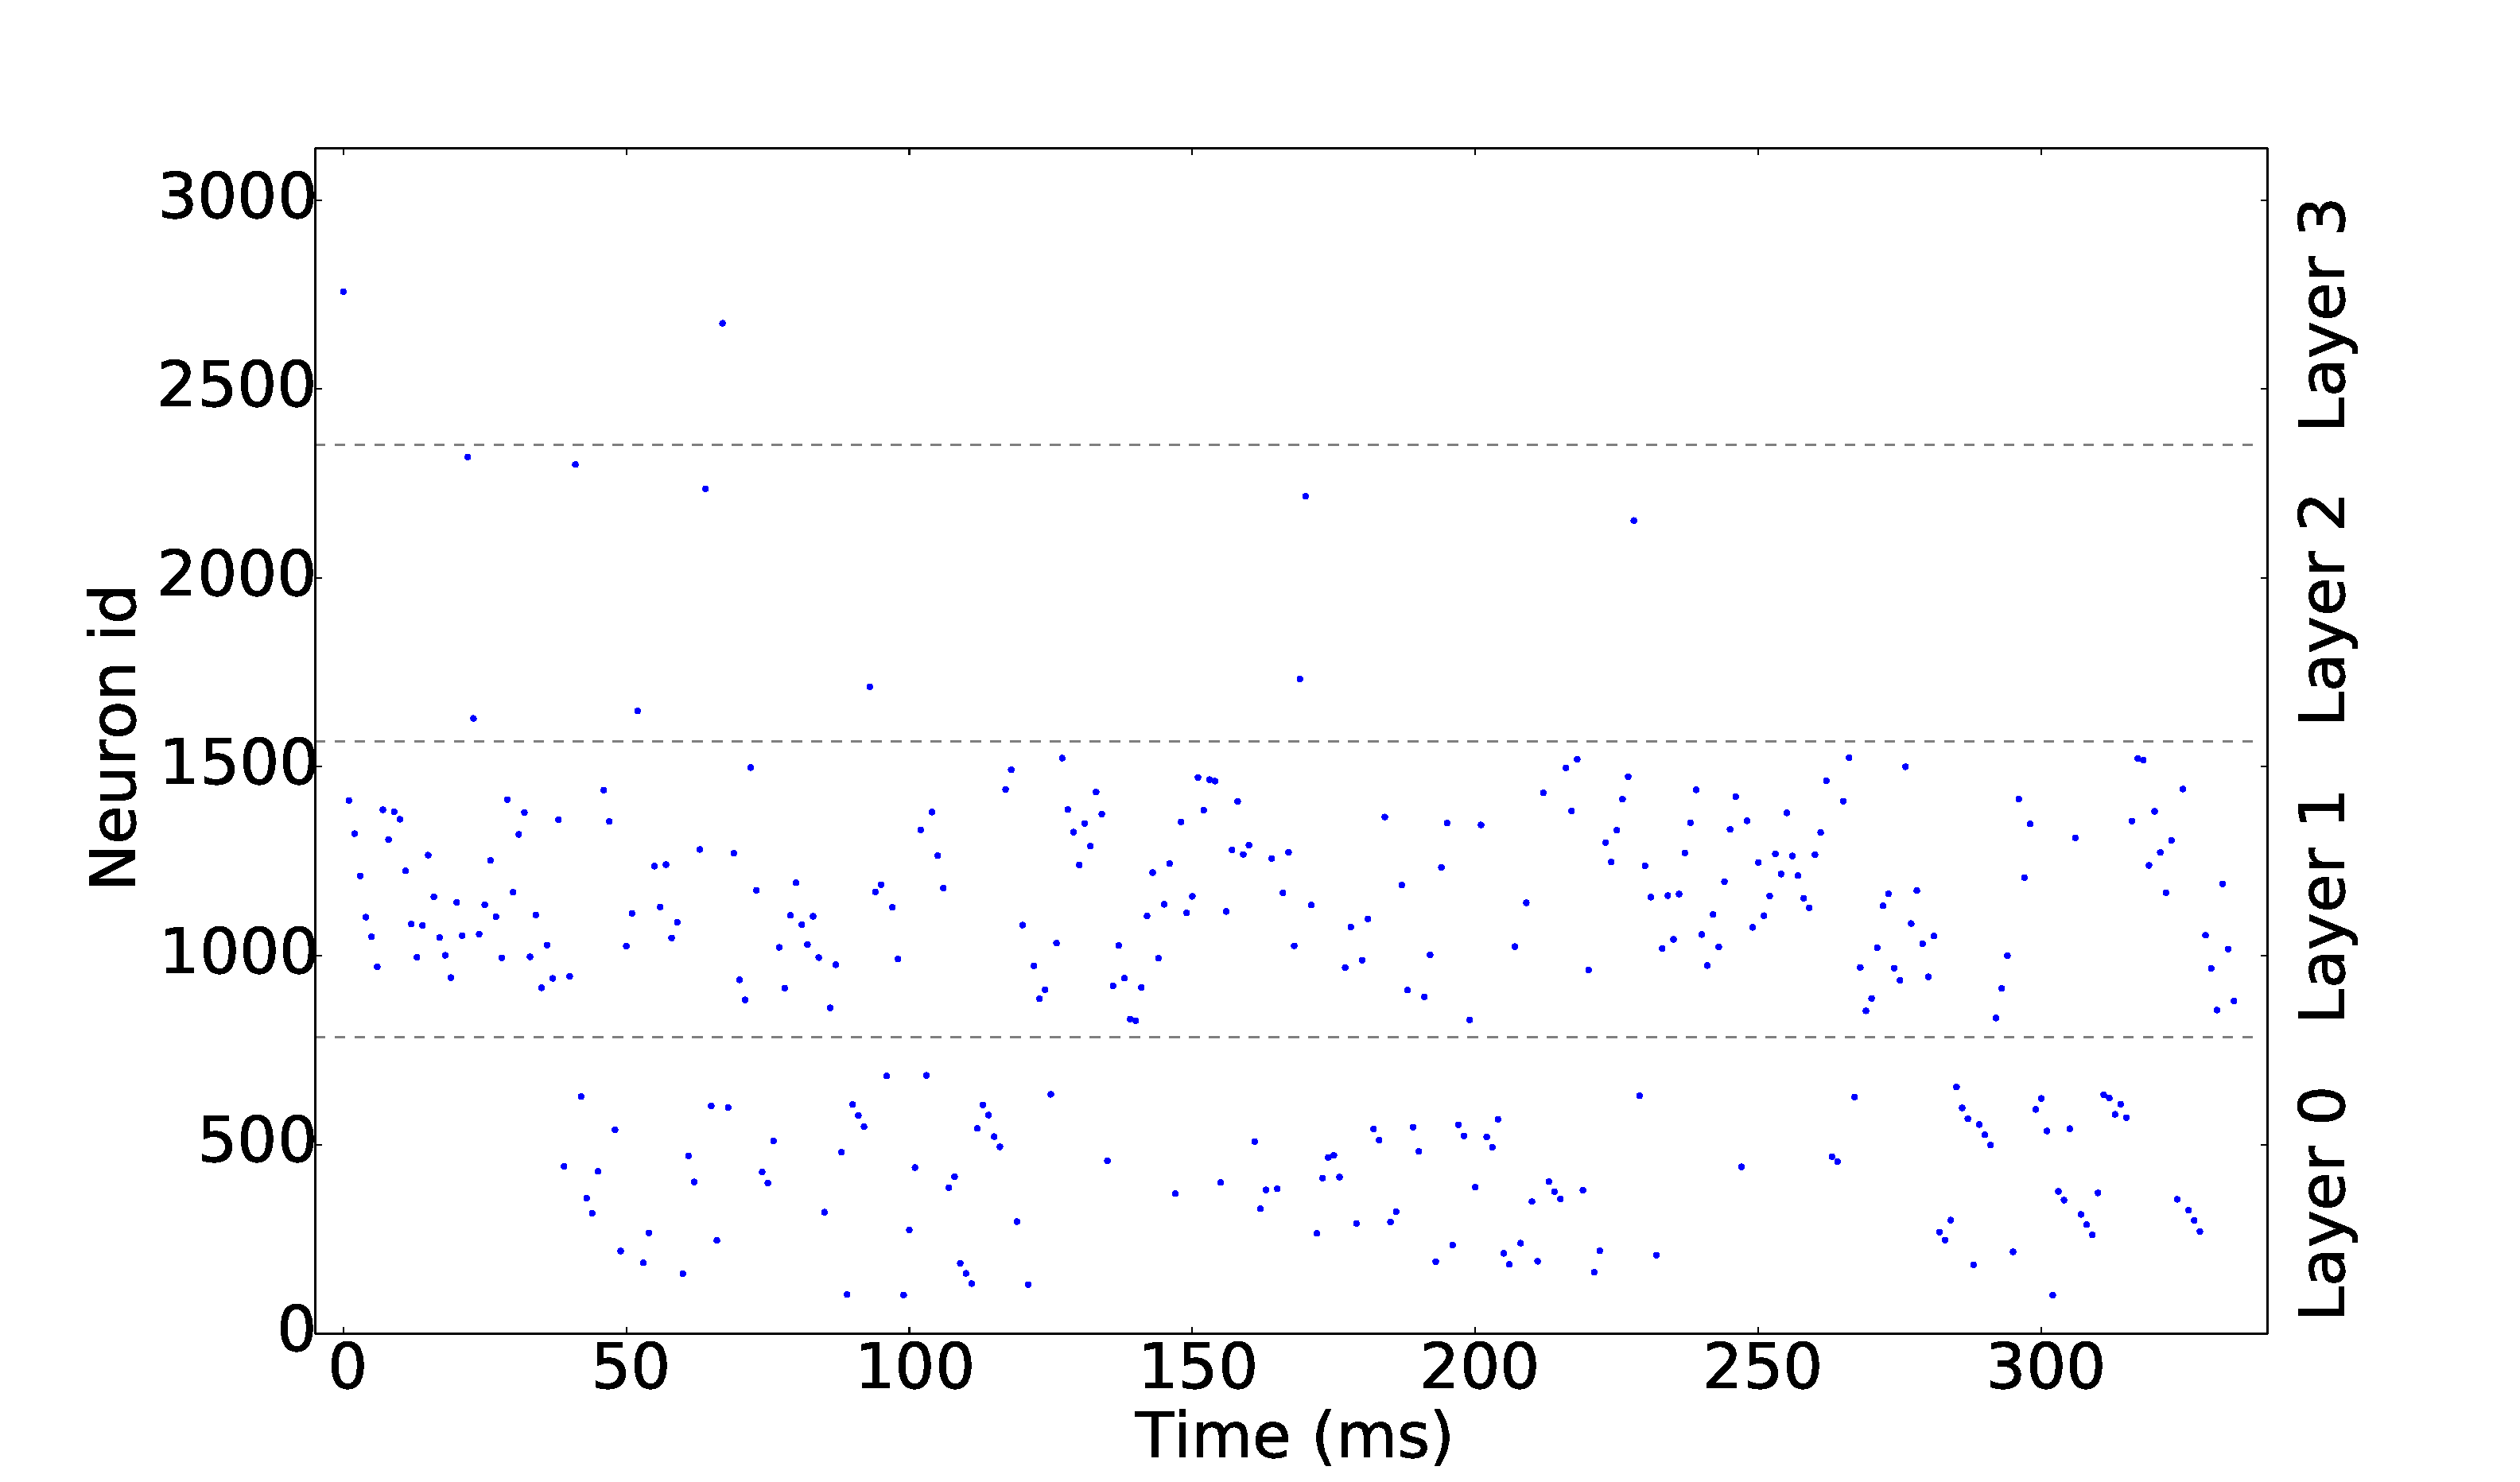
\includegraphics[width=0.475\textwidth]{raster-plot-21-0-30pc}
  }\\[0.1em]
  \subfloat[Spikes are, at most, emited once.]{
    \label{fig-sorted-raster-plot-30pc}
    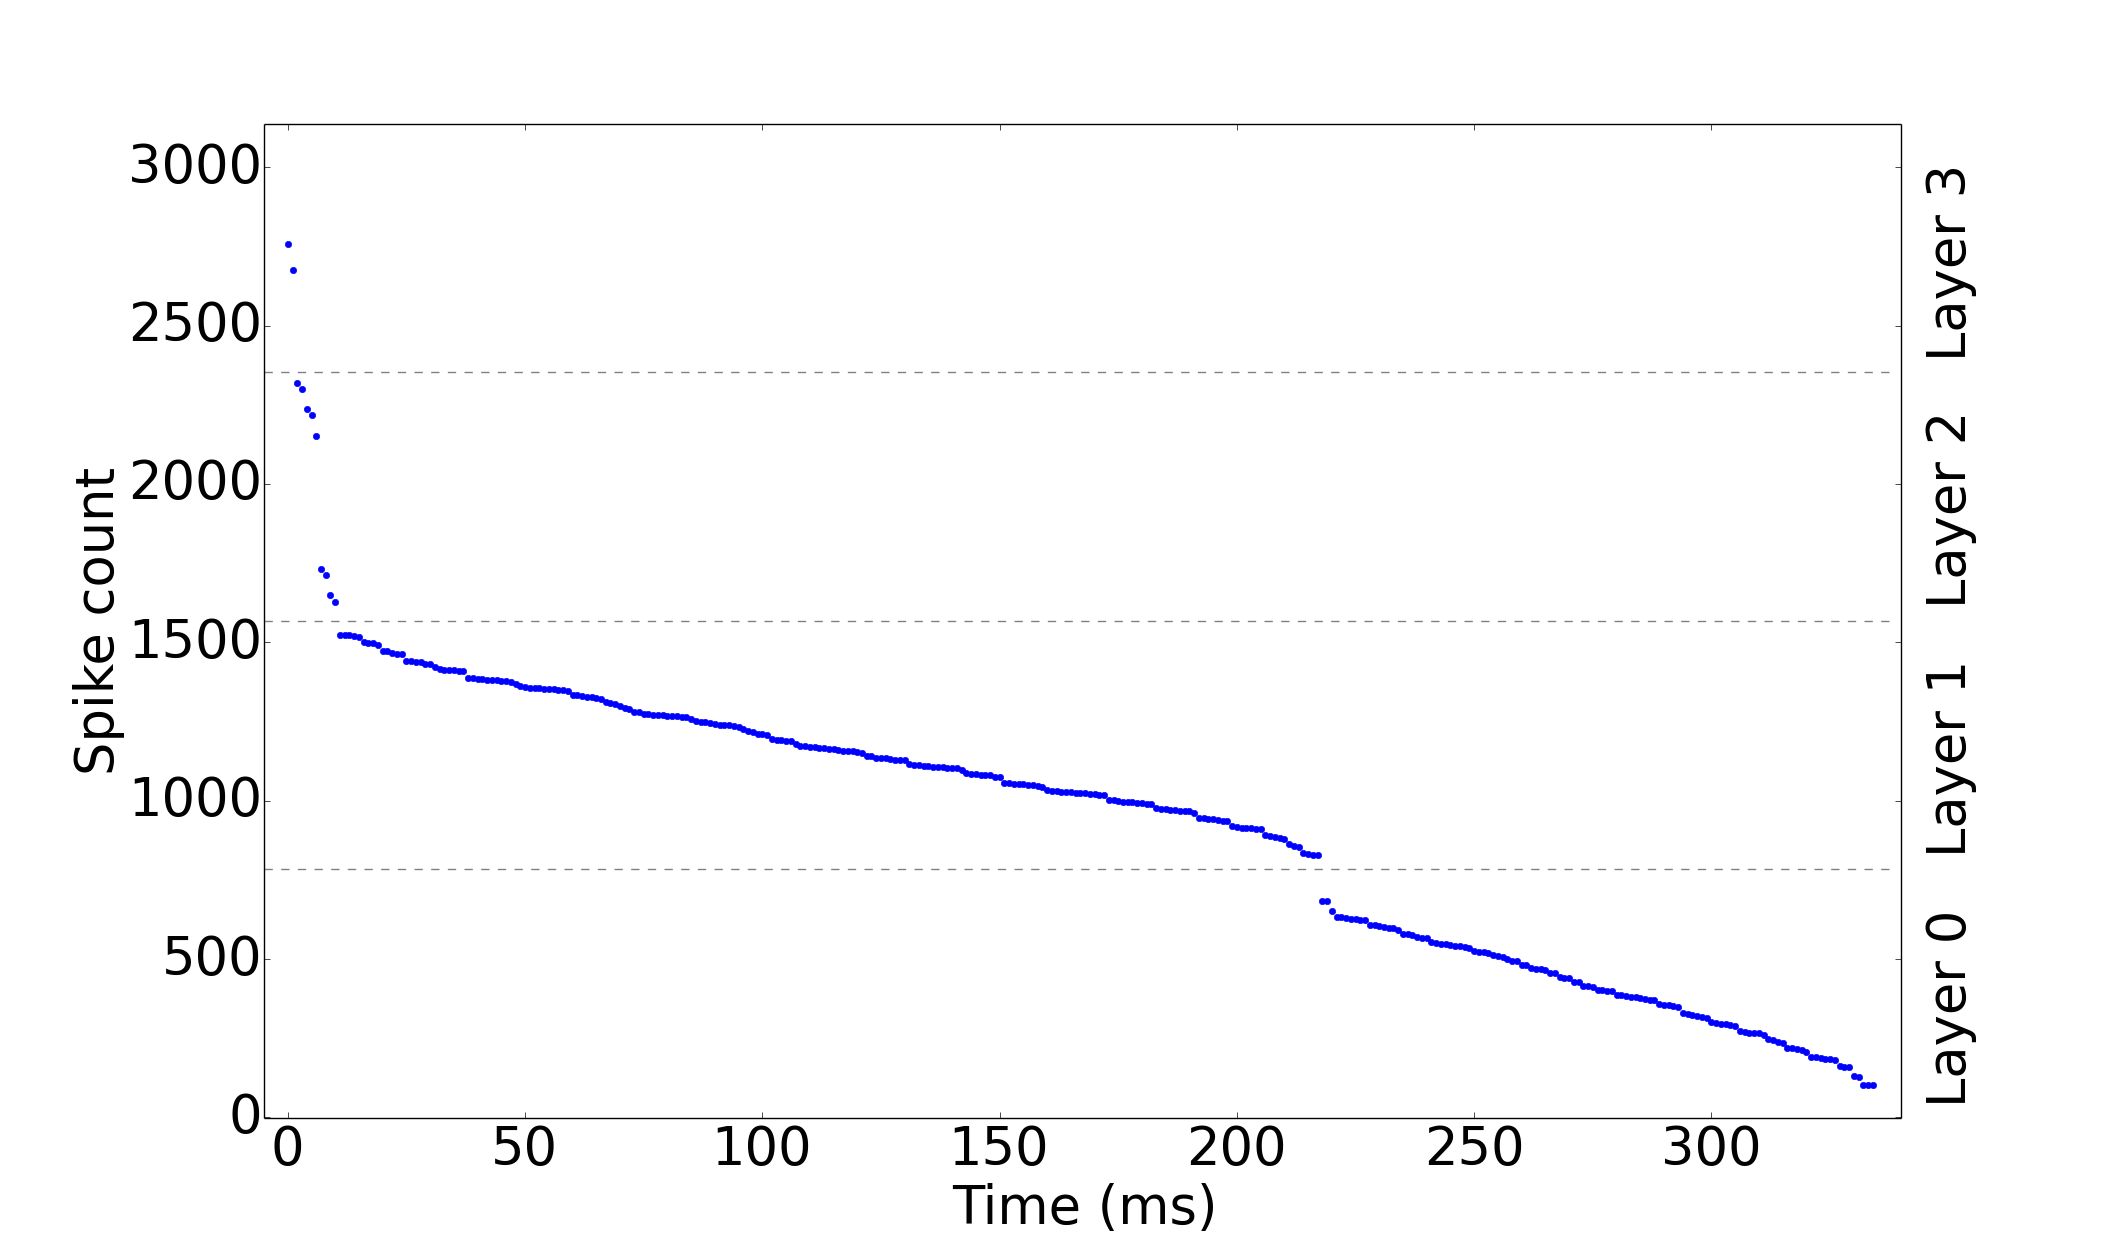
\includegraphics[width=0.475\textwidth]{sorted-raster-plot-21-0-30pc}
  }
  \caption{Analysis of the generated ROC spikes.}
  \label{fig-focal-raster-spikes}
\end{figure}

Figure \ref{fig-reconstruction-results} shows the reconstruction results for the two stages of the algorithm. On Fig. \ref{pic-lena-reconstructed-raw} the reconstruction was applied after the convolution, a blurry image is the result of redundancy in the spike representation. A better reconstruction can be obtained after Algorithm \ref{code-focal-corr} has been performed, the result is shown in Figure \ref{pic-lena-reconstructed-focal}.


\begin{figure}[hbt]
  \centering
  \subfloat[Original image]{
    \label{sfig-rank-ordered-original-1}
    
\includegraphics[width=0.15\textwidth]{original_21-0}
  }
  \subfloat[No correction]{
    \label{pic-lena-reconstructed-raw}
    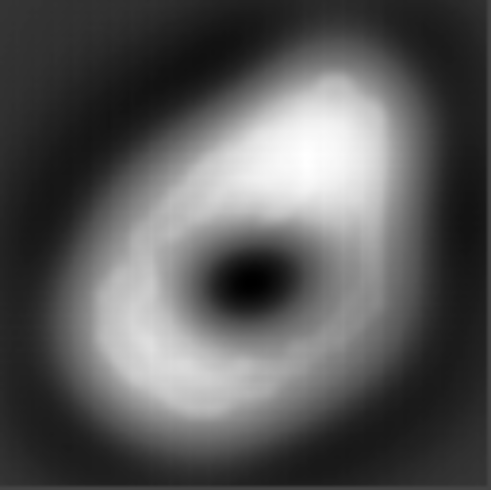
\includegraphics[width=0.15\textwidth]{reconstructed_21-0_raw}
  }
  \subfloat[FoCal]{
    \label{pic-lena-reconstructed-focal}
    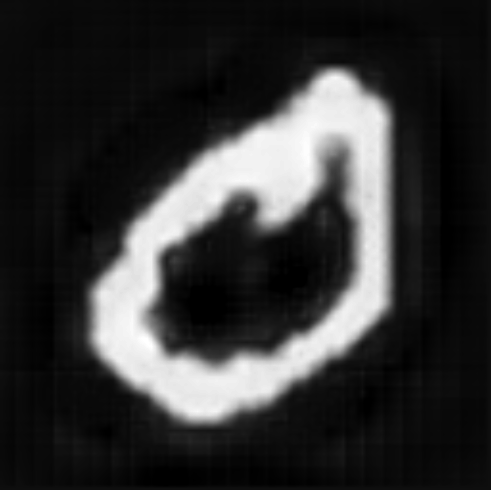
\includegraphics[width=0.15\textwidth]{reconstructed_21-0_100pc}
  }
  \caption{Reconstruction result comparison.}
  \label{fig-reconstruction-results}
\end{figure}
%Two resolutions are provided for the rank-order encoded portion of the database, the first is the original $28\times28$ one. An additional up-scaled resolution version is also provided, the images where scaled to a $128\times128$ resolution using bi-cubic interpolation, this was done to match the DVS native resolution. 

The source Python scripts to transform images to ROC spike trains, to convert the results into AER and pyNN's spike source array will be provided.